%WARNING: amsmath not available

\begin{figure}[!ht]
\begin{ccTexOnly}
\centerline{
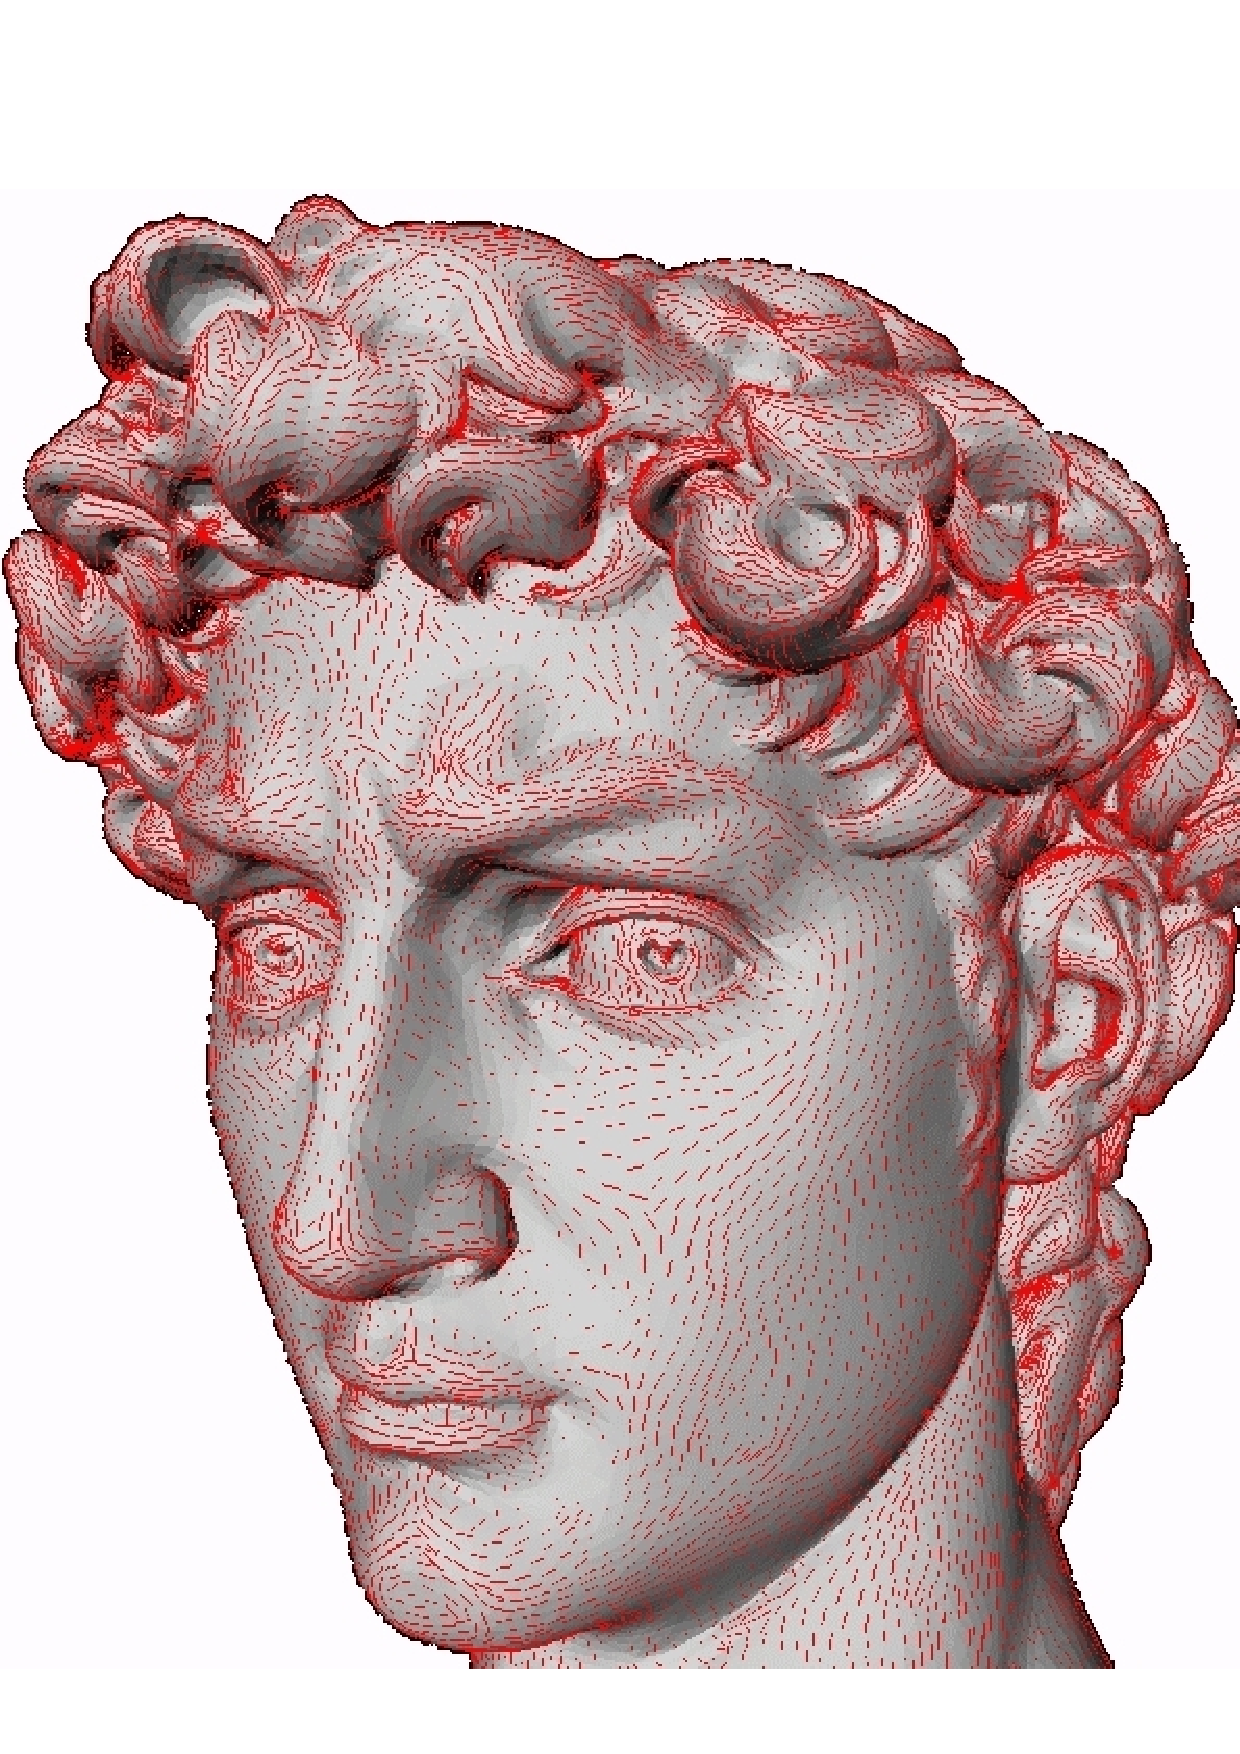
\includegraphics[width=.5\linewidth]{Jet_fitting_3/david-dirmaxkmin-jpg-white-back}}
\end{ccTexOnly}


\begin{ccHtmlOnly}
<CENTER> <img border=0 src="./david-dirmaxkmin-white-back.jpg" width=400>
</CENTER>
\end{ccHtmlOnly}
\caption{Principal directions associated with $k_{max}$ scaled by $k_{min}$.}
\label{fig:jet3:fig-david}
\end{figure}

This package allows the estimation of local differential quantities of
  a surface from a point sample, given either as a mesh or as point
  cloud.

Note that this package needs the third party library
\ccThirdPartyEigen\ to be installed to compile the example code.

%%%%%%%%%%%%%%%%%%%%%%%
\section{Introduction\label{sec:intro}}
%%%%%%%%%%%%%%%%%%%%%%%

\subsection{Overview}
%%%%%%%%%%%%%%%%%%%%%

Consider a sampled smooth surface, and assume we are given a
collection of points $P$ about a given sample $p$. We aim at
estimating the differential properties up to any fixed order of the
surface at point $p$ from the point set $P^+ = P\cup \{ p\}$ --- we
denote $N=\mid P^+\mid$. More precisely, first order properties
correspond to the normal or the tangent plane; second order properties
provide the principal curvatures and directions, third order
properties provide the directional derivatives of the principal
curvatures along the curvature lines, etc.  Most of the time,
estimating first and second order differential quantities is
sufficient.  However, some applications involving shape analysis
require estimating third and fourth order differential quantities.
%%
Many different estimators have been proposed in the vast literature of
applied geometry \cite{cgal:p-smrqt-01} (section 3, page 7), and all
of them need to define a neighborhood around the point at which the
estimation is computed.  Our method relies on smooth differential
geometry calculations, carried out on smooth objects {\em fitted} from
the sample points. 
%%
Datasets amenable to such a processing are naturally unstructured
point clouds, as well as meshes ---whose topological information may
be discarded.

Estimating differential properties from discrete date always raises a
philosophical issue.
%%
On one hand, estimating differential quantities subsumes a smooth
surface does exist.
In this spirit one wishes to recover its differential
properties, so that any estimation method must come with an
asymptotic convergence analysis of the results returned. For the
method developed in this \cgal\ package, the
interested will find such an analysis in
\cite{cgal:cp-edqpf-05}, (Theorem 3)---\ it should be stressed 
the error bounds proved therein are optimal.

On the other hand, any estimation method may be applied to arbitrarily
data ---surface unknown, surface piecewise smooth etc. In such a case,
no analysis can be carried out, and it is up to the users to check the
results match their needs.

%% and only the user can judge if the results are relevant for its use.

Unlike most of the \cgal\ packages, this package uses approximation
methods and is not intended to provide an exact canonical result in
any sense. This is why internal computations are performed with a
number type possibly different from that of the input data, even if
for convenience the results are returned with this original number
type. A reasonable choice for this internal number type is for example
the \ccc{double} type.

\subsection{Smooth Surfaces, $d$-Jets and the Monge Form}
%%%%%%%%%%%%%%%%%%%%%%%%%%%%%%%%

To present the method, we shall need the following notions. Consider a
smooth surface.  About one of its points, consider a coordinate system
whose $z$-axis does not belong to the tangent space. In such a frame,
the surface can locally be written as the graph of a bivariate
function. Letting $h.o.t.$ stand for {\em higher order terms}, one
has~:
%
\begin{equation}
z(x,y)=J_{B,d}(x,y) + h.o.t. \ ; \quad 
J_{B,d}(x,y)=\ccSum{k=0}{d}{(\ccSum{i=0}{i}{
\frac{B_{k-i,i}x^{k-i}y^{i}}{i!(k-i)!}})}.
\end{equation}
The degree $d$ polynomial $J_{B,d}$ is the Taylor expansion of the
function $z$, and is called its {\em $d$-jet}. Notice that a $d$-jet contains
$N_d=(d+1)(d+2)/2$ coefficients.

Recall that an umbilical point of a surface --- or umbilic for short,
is a point where both principal curvatures are identical.  At any
point of the surface which is not an umbilic, principal directions
$d_1, d_2$ are well defined, and these (non oriented) directions
together with the normal vector $n$ define two direct orthonormal
frames. If $v_1$ is a unit vector of direction $d_1$, there exists a
unique unit vector $v_2$ so that $(v_1,v_2,n)$ is direct; and the
other possible frame is $(-v_1,-v_2,n)$.  Both these coordinate
systems are known as the {\em Monge coordinate systems}. In both these
systems, the surface is said to be given in the Monge form and its jet
has the following canonical form~:

\begin{eqnarray}
\label{eq:monge}
z(x,y) =  & \frac{1}{2}(k_1x^2 + k_2y^2)+
	\frac{1}{6}(b_0x^3+3b_1x^2y+3b_2xy^2+b_3y^3) \\
  &  +\frac{1}{24}(c_0x^4+4c_1x^3y+6c_2x^2y^2+4c_3xy^3+c_4y^4) + h.o.t.
\end{eqnarray}

The coefficients $k_1, k_2$ are the principal curvatures,
$b_0,b_3$ are the directional derivatives of $k_1,k_2$ along their
respective curvature line, while $b_1,b_2$ are the directional
derivatives of $k_1,k_2$ along the other curvature lines.

The Monge coordinate system can be computed from any $d$-jet ($d\geq
2$), and so are the Monge coefficients. These informations
characterize the local geometry of the surface in a canonical way, and
are the quantities returned by our algorithm.


\subsection{Algorithm}
%
Based on the above concepts, the algorithm consists of 4 steps.
%
\begin{enumerate}
\item
We perform a Principal Component Analysis (PCA) on $P^+$. This
analysis outputs three orthonormal eigenvectors and the associated
eigenvalues.  The fitting basis consists of these three vectors so
that the vector associated to the smallest eigenvalue is the last
vector of the basis. (Indeed, if the surface is well sampled, one
expects the PCA to provide one small and two large eigenvalues, the
eigenvector associated to the small one approximating the normal
vector.)
\item
We perform a change of coordinates to move the samples into the
coordinate system of the fitting basis and with origin the point $p$
at which the estimation is sought. We then resort to polynomial
fitting, so as to either interpolate or approximate the $d$-jet of the
surface in this coordinate system. This bivariate polynomial
approximation reduces to linear algebra operations.
\item
From the fitted $d$-jet, we compute the Monge basis $(d_1,d_2,n)$.
\item
Finally, we compute the Monge coefficients : $k_i, b_i, c_i$.
\end{enumerate}

Further details can be found in section \ref{sec:details} and in
\cite{cgal:cp-edqpf-05} (section 6).

\subsection{Degenerate Cases\label{sec:deg-cases}}
%%%%%%%%%%%%%%%%%%%%%

As usual, the  fitting procedure may run into (almost) degenerate
cases:
%%
\begin{itemize}
\item Due to poor sampling, the PCA used to determine a rough normal
  vector may not be good. The nearer this direction to the tangent
  plane the worse the estimation.

\item As observed in \cite{cgal:cp-edqpf-05} (section 3.1), the
  interpolating problem is not {\em poised} if the points project,
  into the fitting frame, onto an algebraic curve of degree $d$. More
  generally, the problem is ill poised if the condition number is too
  large.
\end{itemize}
%%
In these cases, even if a result is provided, the estimation may not
be relevant. To inform the user of these issues, we provide the PCA
results and the condition number of the fitting. In any case, it is up
to the user to judge if the result meets its need.


\section{Software Design}
%%%%%%%%%%%%%%%%%%%%%%%

\subsection{Options and Interface Specifications}
%%%%%%%%%%%%%%%%%%%%%

The fitting strategy performed by the class
\ccc{Monge_via_jet_fitting} requires the following parameters:
\begin{itemize}
\item
the degree $d$ of the fitted polynomial ($d \geq 1$),
\item
the degree $d'$ of the Monge coefficients sought, with $1 \leq d' \leq
\min(d,4) $,
\item
a range of $N$ input points on the surface, with the precondition that
$N \geq N_d = (d+1)(d+2)/2$. Note that if $N=N_d$, interpolation
is performed; and if $N >N_d$, approximation is used.
\end{itemize}

\subsection{Output}
%%%%%%%%%%%%%%%%%%%%

As explained in Section \ref{sec:intro}, the output consists of a
coordinate system, the Monge basis, together with the Monge
coefficients which are stored in the \ccc{Monge_form} class. In
addition, more information on the computational issues are stored in
the \ccc{Monge_via_jet_fitting} class.

The \ccc{Monge_form} class provides the following information.

\begin{itemize}
\item Origin. This is the point on the fitted polynomial surface
where the differential quantities have been computed. In the
approximation case, it differs from the input point $p$~: it is the
projection of $p$ onto the fitted surface following the $z$-direction
of the fitting basis.

\item Monge Basis. The Monge basis $(d_1,d_2,n)$ is orthonormal
direct, and the maximal, minimal curvatures are defined wrt this
basis. If the user has a predefined normal $n_0$ (e.g. the sample
points come from an oriented mesh) then if $n_0 . n >0$ then max-min
is correct; if not, i.e. $n_0 . n <0$, the user should switch to the
orthonormal direct basis $(d_1',d_2',n')=(d_2,d_1,-n)$ with the
maximal curvature $k_1'=-k_2$ and the minimal curvature
$k_2'=-k_1$. If $n_0 . n =0$ or is small, the orientation of the
surface is clearly ill-defined, and the user may proof-check the
samples used to comply with its predefined normal.

%% then this means that the orientation of the surface is not so clear!

\item Monge Coefficients.
The coefficient of the Monge form is $(k_1, k_2 (\leq k_1),
b_0, b_1, b_2, b_3, c_0, c_1, c_2, c_3, c_4)$ for $d' = 4$.

\end{itemize}

In addition, the class \ccc{Monge_via_jet_fitting} stores 
\begin{itemize}
\item
the condition number of the fitting system,
\item 
the coordinate system of the PCA (in which the fitting is performed).
\end{itemize}

\subsection{Template Parameters}
%%%%%%%%%%%%%%%%%%%%%%%%%%%%%%%%%

\subsubsection{Template parameter \texttt{DataKernel}}
%%%%%%%%%%%

This concept provides the types for the input sample points, together
with $3d$ vectors and a number type. It is used as template for the
class \ccc{Monge_via_jet_fitting<DataKernel, LocalKernel, SvdTraits>} . Typically, one can use
\ccc{CGAL::Cartesian<double>}.

\subsubsection{Template parameter \texttt{LocalKernel}}
%%%%%%%%%%%
This is a parameter of the class 
\ccc{Monge_via_jet_fitting<DataKernel, LocalKernel, SvdTraits>}. 
This concept defines the vector and number types used for local
computations and to store the PCA basis data.  

Input points of type
\ccc{DataKernel::Point_3} are converted to
\ccc{LocalKernel::Point_3}. For output of the \ccc{Monge_form} class,
these types are converted back to \ccc{Data_Kernel} ones.  Typically,
one can use
\ccc{CGAL::Cartesian<double>} which is the default.

\subsubsection{Template parameter \texttt{SvdTraits}}
%%%%%%%%%%%

This concept provides the number, vector and matrix types for algebra
operations required by the fitting method in
\ccc{Monge_via_jet_fitting<DataKernel, LocalKernel, SvdTraits>} 
. The main method is a linear solver using a singular value decomposition.

\subsubsection{Compatibility requirements}
%%%%%%%%%%%

To solve the fitting problem, the sample points are first converted
from the \ccc{DataKernel} to the \ccc{LocalKernel} (this is done using
the \ccc{CGAL::Cartesian_converter}). Then change of coordinate
systems and linear algebra operations are performed with this
kernel. This implies that the number types \ccc{LocalKernel::FT} and
\ccc{SvdTraits::FT} must be identical.
Second the Monge basis and coefficients, computed with the
\ccc{LocalKernel}, are converted back to the \ccc{DataKernel} 
(this is done using the \ccc{CGAL::Cartesian_converter} and the
\ccc{CGAL::NT_converter}).


\section{Examples} 
%%%%%%%%%%%%%%%%%%%%%%%%%%%%%%%%%%%%%%%%%%%%%%%%%%%%%%%%%%%%%%%%%%%%%%%%%%%%

\subsection{Single Estimation about a Point of a Point Cloud}

The first example illustrates the computation of the local
differential quantities from a set of points given in a text file as
input. The first point of the list is the one at which the computation
is performed. The user has to specify a file for the input points and
the degrees $d$ and $d'$.
\ccIncludeExampleCode{Jet_fitting_3/Single_estimation.cpp}

\subsection{On a Mesh}
The second example (cf Mesh\_estimation.cpp in the example directory)
illustrates the computation of local differential quantities for all
vertices of a given mesh. The neighborhood of a given vertex is
computed using rings on the triangulation. Results are twofold:
\begin{itemize}
\item a human readable text file featuring the \ccc{Monge_form} and
  numerical informations on the computation~: condition number and the
  PCA basis;
\item another text file that records raw data (better for a vizualization
   post-processing).
\end{itemize}


%%Following are some illustrations featuring principal directions of curvature.

Figs.
\ref{fig:jet3:fig-david} and
\ref{fig:jet3:fig-elliptic-paraboloid}
provide illustrations of principal directions of curvature.

% \begin{figure}[!ht]
% \begin{ccTexOnly}
% \centerline{
% 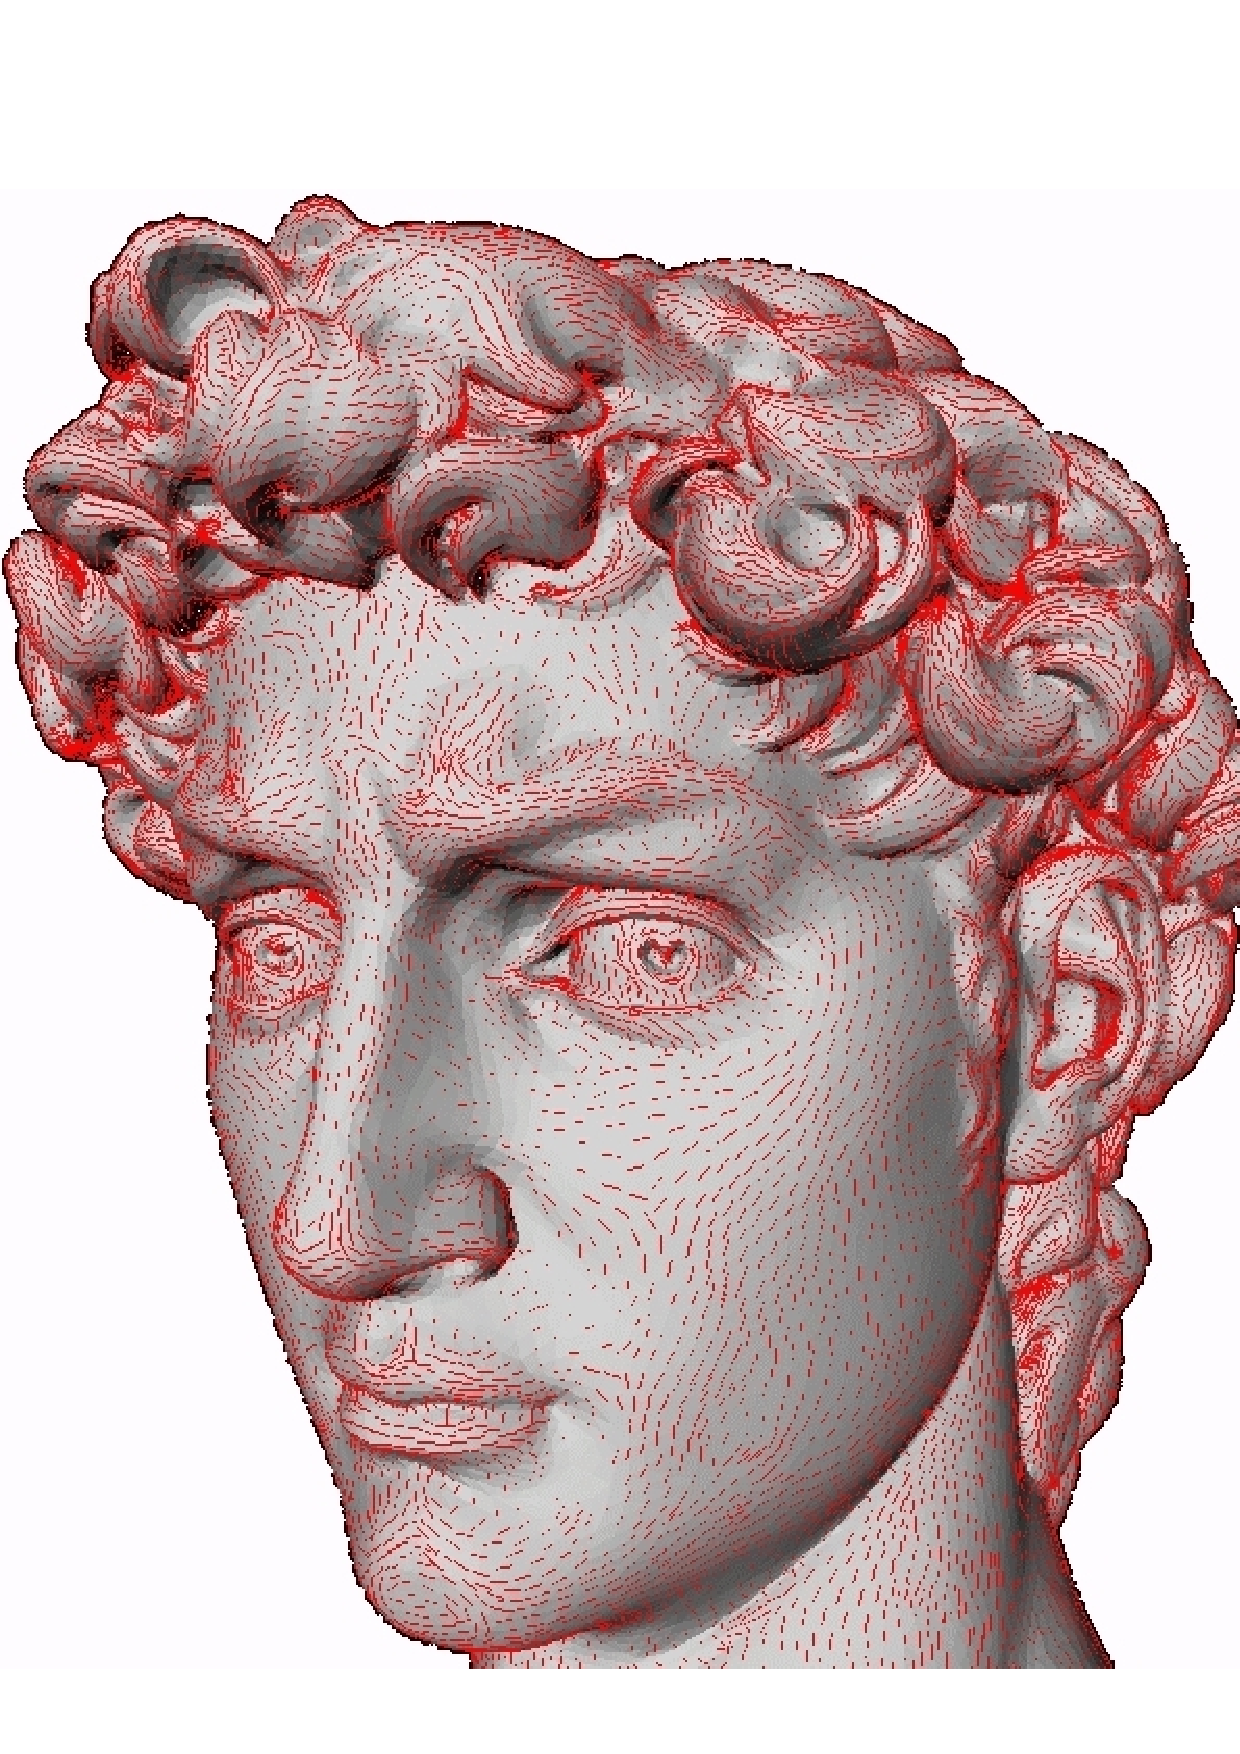
\includegraphics[width=.5\linewidth]{Jet_fitting_3/david-dirmaxkmin-jpg-white-back}}
% \end{ccTexOnly}
% \caption{Principal directions associated with $k_{max}$ scaled by $k_{min}$.}

% \begin{ccHtmlOnly}
% <CENTER> <img border=0 src="./david-dirmaxkmin-white-back.jpg" width=600>
% </CENTER>
% \end{ccHtmlOnly}
% \label{fig:jet3:fig-david}
% \end{figure}

 

\begin{figure}[!ht]
\begin{ccTexOnly}
\centerline{
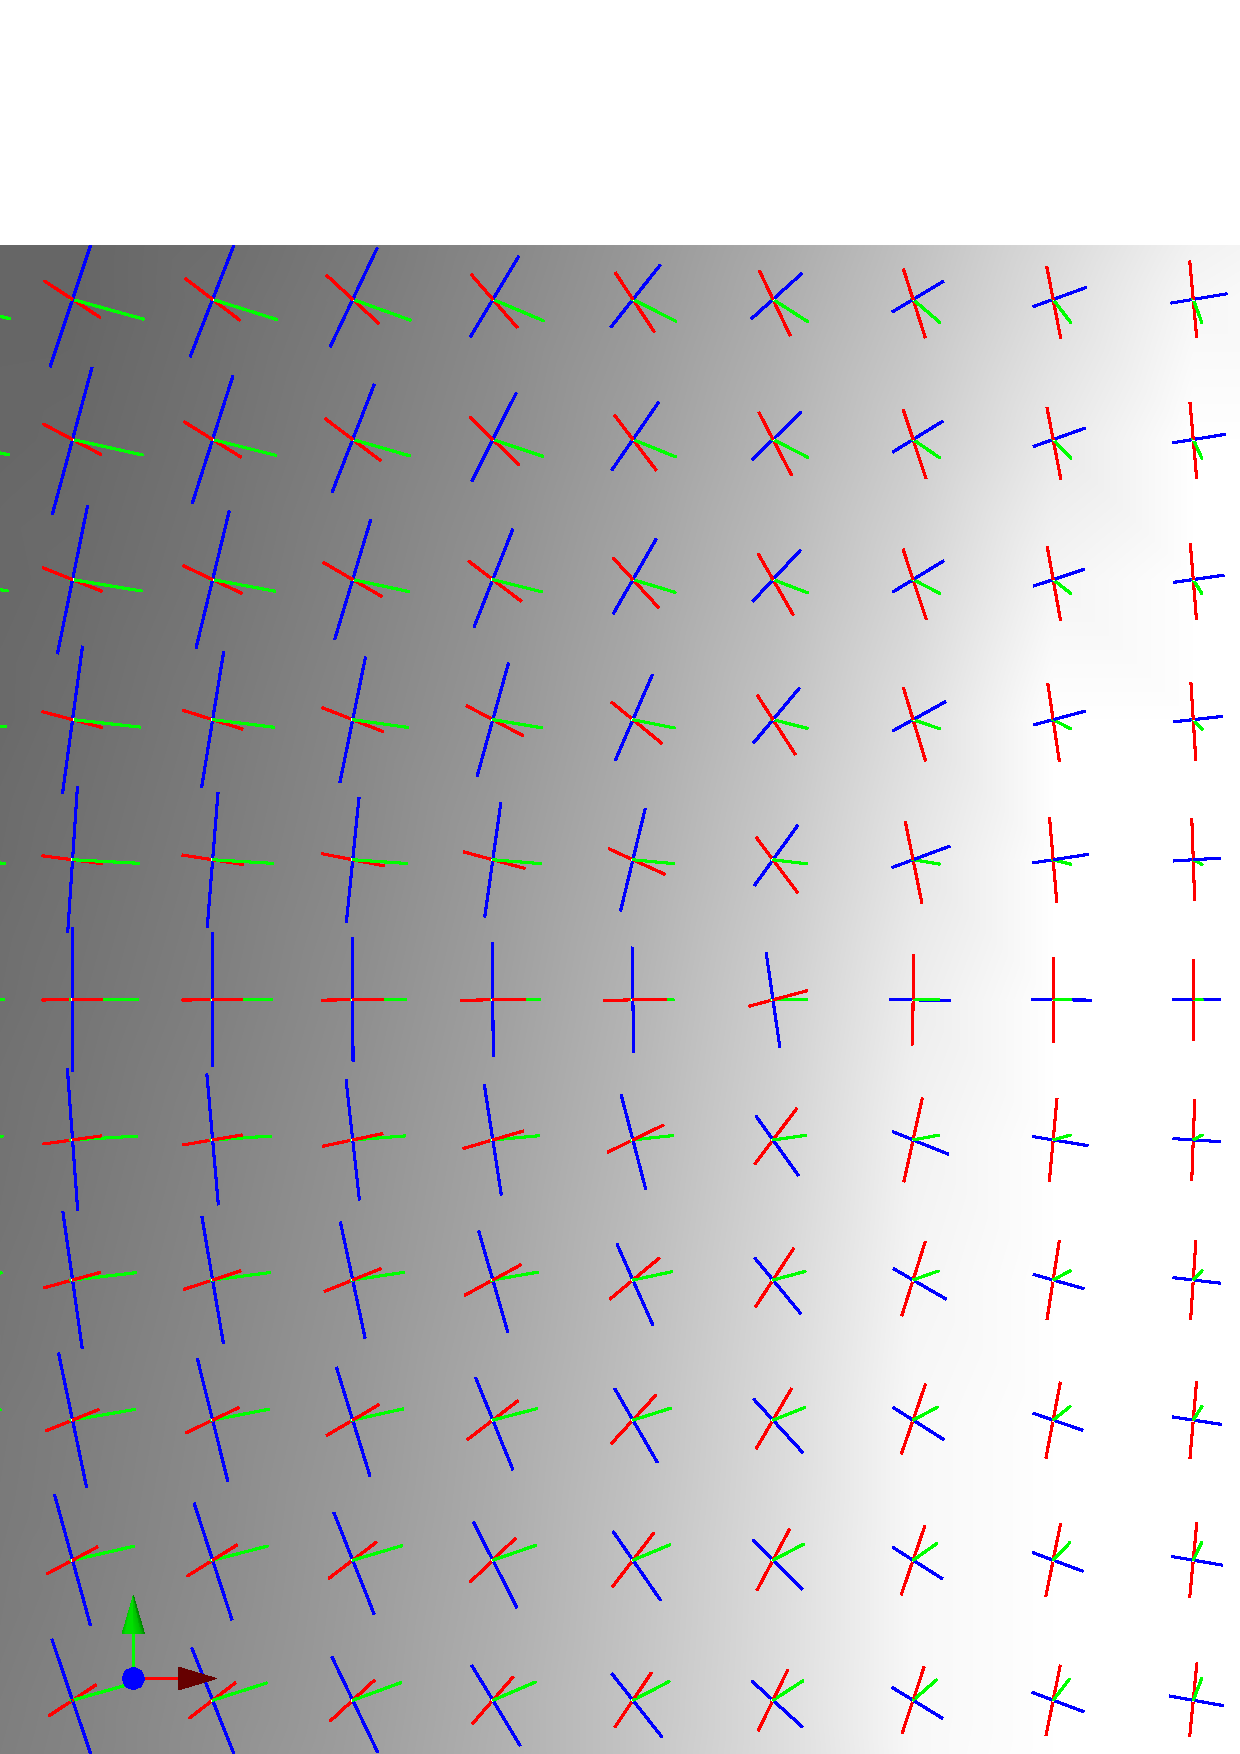
\includegraphics[width=.5\linewidth]{Jet_fitting_3/ppal_curv_poly2x2+y2}}
\end{ccTexOnly}

\begin{ccHtmlOnly}
<CENTER> <img border=0 src="./ppal_curv_poly2x2+y2.jpg" width=600>
</CENTER>
\end{ccHtmlOnly}
\caption{Principal directions of curvature and normals at vertices of a mesh of the
 graph of the function $f(x,y)=2x^2+y^2$.}
\label{fig:jet3:fig-elliptic-paraboloid}
\end{figure}
  
 \begin{ccAdvanced} 
\section{Mathematical and Algorithmic Details}
%%%%%%%%%%%%%%%%%%%%%%%
\label{sec:details}
In this Section, we detail the mathematics involved, in order to
justify the design choices made.
%%
To begin with, observe the fitting problem involves three relevant
direct orthonormal basis: the world-basis $(w_x,w_y,w_z)$, the
fitting-basis $(f_x,f_y,f_z)$, the Monge basis $(d_1,d_2,n)$.

\begin{figure}[!ht]
\begin{ccTexOnly}
\centerline{
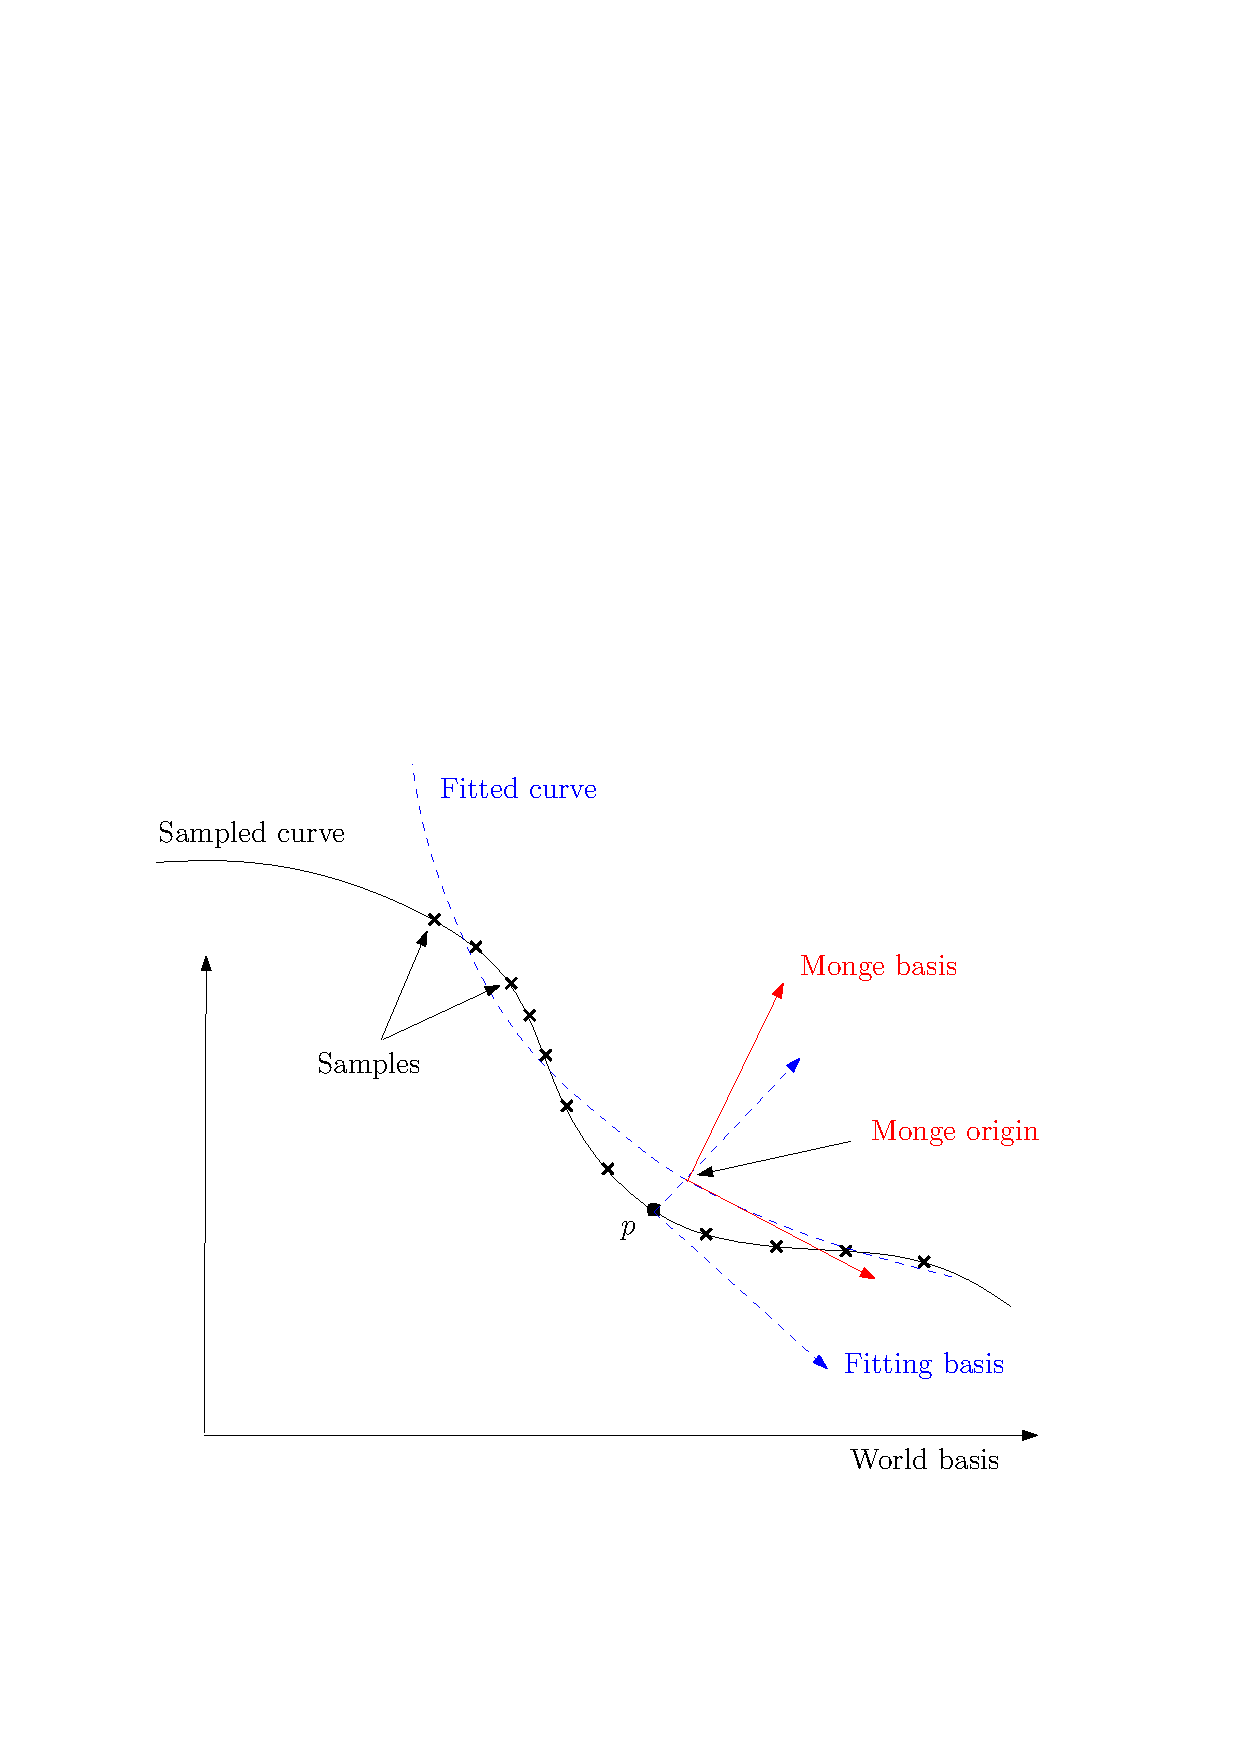
\includegraphics[width=.5\linewidth]{Jet_fitting_3/jet_fitting_basis}}
\end{ccTexOnly}

\label{fig:jet_fitting_basis}

\begin{ccHtmlOnly}
<CENTER>
<img border=0 src="./jet_fitting_basis.gif" width=600>
</CENTER>
\end{ccHtmlOnly}
\caption{The three bases involved in the estimation.}
\end{figure}

\subsection{Computing a Basis for the Fitting}
%%%%%%%%%%%%%%%%%%%%%%%%%%%%%%%%%%%%%%%%%%%%%%%%%%%%%%%%%%%%%

{\bf Input : samples\\ Output : fitting-basis}


%, and we
%shall assume a function {\tt eigen\_symm\_algo} doing so is available.
%
%a Principal Component Analysis, this means we need a linear
%algebra method to perform an eigen analysis of a symmetric matrix :
%{\tt eigen\_symm\_algo}. 
%
Performing a PCA requires diagonalizing a symmetric matrix.  This
analysis gives an orthonormal basis whose $z$-axis is provided by the
eigenvector associated to the smallest eigenvalue.\footnote{Another
  possibility is to choose as z-axis the axis of the world-basis with
  the least angle with the axis determined with the PCA. Then the
  change of basis reduces to a permutation of axis.} Note one may have
to swap the orientation of a vector to get a direct basis.

Let us denote $P_{W\rightarrow F}$ the matrix that changes coordinates from the
world-basis $(w_x,w_y,w_z)$ to the fitting-basis $(f_x,f_y,f_z)$. The
rows of $P_{W\rightarrow F}$ are the coordinates of the vectors
$(f_x,f_y,f_z)$ in the world-basis. This matrix represents a
orthogonal transformation hence its inverse is its transpose. To obtain
the coordinates of a point in the fitting-basis from the coordinates
in the world-basis, one has to multiply by $ P_{W\rightarrow F}$.

As mentioned above, the eigenvalues are returned, from which the
sampling quality can be assessed. For a good sampling, the eigenvector
associated to the smallest eigenvalue should roughly give the normal
direction.

\subsection{Solving the Interpolation / Approximation Problem\label{sec:solving}}
%%%%%%%%%%%%%%%%%%%%%%%%%%%%%%%%%%%%%%%%%%%%%%%%%%%%%%%%%%%%%

{\bf Input : samples, fitting-basis \\ Output : coefficients $A_{i,j}$
of the bivariate fitted polynomial in the fitting-basis }

Computations are done in the fitting-basis and the origin is the point
$p$. First, one has to transform coordinates of sample points with a
translation ($-p$) and multiplication by $ P_{W\rightarrow F}$.

The fitting process consists of finding the coefficients
$A_{i,j}$ of the degree $d$ polynomial 
\begin{equation}
\label{eq-answer}
J_{A,d}= \ccSum{k=0}{d}{(\ccSum{i=0}{k}{
\frac{A_{k-i,i}x^{k-i}y^{i}}{i!(k-i)!}})}.
\end{equation}


Denote $p_i=(x_i,y_i,z_i), \ i=1,\ldots , N$ the coordinates of the
sample points of $P^+$.
%%
For interpolation the linear equations to solve are $A(x_i,y_i)=z_i \
i=1,\ldots,N$, and for approximation one has to minimize $\sum_{i=1}^N
(A(x_i,y_i)-z_i)^2$. The linear algebra formulation of the problem is
given by
%
\begin{eqnarray}
\label{eq:fit-linalg}
 A =  & (A_{0,0}, A_{1,0},A_{0,1}, \ldots , A_{0,d})^T \\ 
 Z=  &(z_1, z_2,\ldots , z_N)^T \\ 
 M=  &(1,x_i,\ y_i,\ \frac{x_i^2}{2},\ldots ,
\ \frac{x_iy_i^{d-1}}{(d-1)!},\ \frac{y_i^d}{d!})_{i=1,...,N}\\
\end{eqnarray}
%
The equations for interpolation become $MA=Z$. For approximation, the
system $MA=Z$ is solved in the least square sense, i.e. one seeks the
vector $A$ such that $A = \arg \min_A ||MA-Z||_2$.

In any case, there is a preconditioning of the matrix $M$ so as to
improve the condition number. Assuming the $\{x_i\}$, $\{y_i\}$ are of
order $h$, the pre-conditioning consists of performing a column
scaling by dividing each monomial $x_i^ky_i^l$ by $h^{k+l}$ --- refer
to Eq. (\ref{eq:fit-linalg}). Practically, the parameter $h$ is chosen
as the mean value of the $\{x_i\}$ and $\{y_i\}$. In other words, the
new system is $M'Y=(MD^{-1})(DA)=Z$ with $D$ the diagonal matrix
$D=(1,h,h,h^2,\ldots,h^d,h^d)$, so that the solution $A$ of the
original system is $A=D^{-1}Y$.

There is always a single solution since for under constrained systems
we also minimize $||A||_2$.  The method uses a singular value
decomposition of the $N\times N_d$ matrix $M= U S V^T$, where $U$ is a
$N \times N$ orthogonal matrix, $V$ is a $N_d \times N_d$ orthogonal
matrix and $S$ is a $N\times N_d$ matrix with the singular values on
its diagonal. Denote $r$ the rank of $M$, we can decompose
%
$S= \left( \begin{array}{cc}
D_r & 0_{r,\ N_d-r}\\
0_{N-r,\ r} & 0_{N-r,\ N_d-r}
\end{array} 
\right).
$
%
The number $r$, which is the number of non zero singular values, is
strictly lower than $N_d$ if the system is under constrained. In any
case, the unique solution which minimize $||A||_2$ is given by~:
\begin{equation}
A= V
\left( \begin{array}{cc}
D_r^{-1} & 0_{N_d-r,\ r}\\
0_{r,\ N-r} & 0_{N_d-r,\ N-r}
\end{array} 
\right)
 U^TZ.
\end{equation}
%%
One can provide the condition number of the matrix $M$ (after
preconditioning) which is the ratio of the maximal and the minimal
singular values. It is infinite if the system is under constrained,
that is the smallest singular value is zero.

\paragraph{Implementation details.}
We assume a \ccc{solve} function is provided by the traits
\ccc{SvdTraits}. This function solves the system MX=B (in the least square sense
if M is not square) using a Singular Value Decomposition and gives the
condition number of M. 

\medskip
Remark: as an alternative, other methods may be used to solve the
system. A $QR$ decomposition can be substituted to the $SVD$. One can
also use the normal equation $M^TMX=MTB$ and apply methods for square
systems such as $LU$, $QR$ or Cholesky since $M^TM$ is symmetric
definite positive when $M$ has full rank. 
%LU suitable for any square M
%QR for rectangular
%Choleski for symm def + =LL^t
The advantages of the $SVD$
is that it works directly on the rectangular system and gives the
condition number of the system. For more on these alternatives, see
\cite{gl-mc-83} (Chap. 5).

\subsection{Principal  Curvature / Directions}
%%%%%%%%%%%%%%%%%%%%%%%%%%%%%%%%%%%%%%%%%%%%%%

{\bf Input : coefficients of the fit $A_{i,j}$, 
fitting-basis \\
Output : Monge basis wrt fitting-basis and world-basis
}

In the fitting basis, we have determined a height function expressed
by Eq. (\ref{eq-answer}). Computations are done in the fitting-basis.
The partial derivatives, evaluated at $(x,y)=(0,0)$, of the fitted
polynomial $J_{A,d}(x,y)$ are
$A_{i,j}=\frac{\partial^{i+j}J_{A,d}}{\partial^ix \partial^jy}$
%%
Expanding Eq. (\ref{eq-answer}) yields:
%%
\begin{eqnarray}
J_{A,d}(x,y)&=
A_{0,0}+A_{1,0}x+A_{0,1}y+\frac{1}{2}(A_{2,0}x^2+2A_{1,1}xy+A_{0,2}y^2) 
+ \frac{1}{6}(A_{3,0}x^3+3A_{2,1}x^2y+\ldots )+ \ldots 
\end{eqnarray}

\begin{itemize}
\item The origin, that is the point of the fitted surface where the
  estimation is performed, is $(0,0,A_{0,0})$. 
\item The normal is
  $n=(-A_{1,0},-A_{0,1},1)/\sqrt{A_{1,0}^2+A_{0,1}^2+1}$.
\item Curvature related properties are retrieved resorting to
  standard differential calculus \cite{c-dgcs-76} (Chap. 3). More precisely, the
  Weingarten operator $W=-I^{-1}II$ is first computed in the basis of
  the tangent plane $\{ (1,0,A_{1,0}), (0,1,A_{0,1}) \}$. We compute
  an orthonormal basis of the tangent plane using the Gram-Schmidt
  algorithm, and then we compute Weingarten in this basis (applying a
  change of basis with the matrix $W'=P^{-1}WP$). In this orthonormal
  basis, the matrix of the Weingarten map is symmetric and we
  diagonalize it.  One finally gets the principal curvatures which are
  the eigenvalues of $W$, and the associated principal
  directions. This gives an orthonormal direct basis
  $(d_1,d_2,n)$. Let us denote $P_{F \rightarrow M}$ the matrix to
  change coordinates from the fitting-basis to the Monge basis. Its
  rows are the coordinates of the vectors $(d_1,d_2,n)$ in the
  fitting-basis. It is an orthogonal matrix $P_{F \rightarrow
    M}^{-1}=P_{F \rightarrow M}^T$. The Monge basis expressed in the
  world-basis is obtained by multiplying the coordinates of
  $(d_1,d_2,n)$ in the fitting-basis by $P_{W\rightarrow F}^{-1}$,
  (the same holds for the origin point which has in addition to be
  translated by $p$, i.e. the coordinates of the origin point are
  $P_{W\rightarrow F}^{-1} (0,0,A_{0,0}) +p$.
\end{itemize}

\subsection{Computing  Higher Order Monge Coefficients}

{\bf Input : coefficients of the fit, Monge basis wrt fitting-basis ($P_{F
\rightarrow M}$)\\ 
Output : third and fourth order coefficients of Monge}

We use explicit formula. The implicit equation of the fitted
polynomial surface in the fitting-basis with origin the point
$(0,0,A_{0,0})$ is $Q=0$ with
\begin{equation}
Q=-w-A_{0,0}  +\ccSum{i,j}{}{\frac{A_{i,j}u^iv^j}{i!j!}}.
\end{equation}
%%
The equation in the Monge basis is obtained by substituting $(u,v,w)$
by $P^T_{F\rightarrow M}(x,y,z)$. Denote $f(x,y,z)=0$ this implicit
equation. By definition of the Monge basis, we have locally (at
$(0,0,0)$)
\begin{equation}
f(x,y,z)=0 \Leftrightarrow z=g(x,y)
\end{equation}
and the Taylor expansion of $g$ at $(0,0)$ are the Monge coefficients
sought.
%
Let us denote the partial derivatives evaluated at the origin of $f$
and $g$ by $f_{i,j,k}=\frac{\partial^{i+j+k}f}{\partial^ix
\partial^jy \partial^kz}$ and $g_{i,j}=\frac{\partial^{i+j}g}{\partial^ix
\partial^jy}$. One has $f_{1,0,0}=f_{0,1,0}=f_{1,1,0}=0$,
$g_{0,0}=g_{1,0}=g_{0,1}=g_{1,1}=0$ and $g_{2,0}=k_1$,
$g_{0,2}=k_2$. The partial derivative of order $n$ of $f$ depends on
the matrix $P_{F\rightarrow M}$ and the partial derivatives of order
at most $n$ of $J_{A,d}$. The third and fourth order coefficients of are
computed with the implicit function theorem. For instance~:
\begin{eqnarray*}
%&b_0=g_{3,0}=-(f_{3,0,0}-3f_{1,0,1}f_{2,0,0}/f_{0,0,1})/f_{0,0,1}\\
%&b_3=g_{0,3}=-(f_{0,3,0}-3f_{0,1,1}f_{0,2,0}/f_{0,0,1})/f_{0,0,1}\\
%&c_0=g_{4,0}=-(f_{4,0,0}+3f_{2,0,1}g_{2,0}+f_{0,0,2}g_{2,0}^2
%+4f_{1,0,1}g_{30})/f_{0,0,1}\\
%&c_4=g_{0,4}=-(f_{0,4,0}+3f_{0,2,1}g_{0,2}+f_{0,0,2}g_{0,2}^2
%+4f_{0,1,1}g_{0,3})/f_{0,0,1}\\
&b_0=g_{3,0}=-{\frac { f_{3,0,0} f_{0,0,1} -3\, f_{1,0,1} f_{2,0,0} }{
f_{0,0,1} ^{2}}}
\\
&b_1=g_{2,1}=-{\frac {-  f_{0,1,1}      f_{2,0,0}    +  f_{2,1,0}    f_{0,0,1}  }{  f_{0,0,1}    ^{2}}}
\\
& .... \\
\end{eqnarray*} 
 \end{ccAdvanced} 
